\subsection{Test 4:}

For the same graph of Figure 4.3.0, we will analyze the certificate {\itshape C = [ 1, 2, 3, 4, 5, 6, 7, 7, 1 ]}, as we can see clearly, this isn't a {\bfseries Hamiltonial-Cycle} because has a repeated vertex which it's the node 7, so, the program will stop analyzing and will only print on the console output ( Figure 4.4.0 ) that the certificate isn't a {\bfseries Hamiltonial-Cycle}. \hfill \break

\begin{lstlisting}
def main ( ):
    graph = { 1: [ 2, 4, 8 ], 2: [ 7, 3, 1 ], 3: [ 2, 6, 4 ],
              4: [ 1, 3, 5 ], 5: [ 4, 8, 6 ], 6: [ 5, 3, 7 ],
              7: [ 6, 2, 8 ], 8: [ 7, 5, 1 ] }
    certificate = [ 1, 2, 3, 4, 5, 6, 7, 7, 1 ]
    verify_hamiltonian ( graph, certificate )
\end{lstlisting} \hfill \break

\begin{figure}[H]
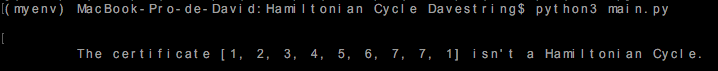
\includegraphics[height = 1.5cm, width = 16.5cm]{13c.png}
\centering \linebreak \linebreak {\small Figure 4.4.0: Console output.}
\end{figure}

\pagebreak